%% !TeX TS-program = pdflatex
%% !BIB TS-program = bibtex
%% !TeX spellcheck = en_US
%%%%%%%%%%%%%%%%%%%%%%%%%%%%%%%%%%%%%%%%%%%%%%%%%%%%%%%%%%%%%%%%%%%%%
%% Many modern TeX editors understand the above lines to overwrite  %
%% globally set settings for individual documents. Just leave one   %
%% percent sign at the beginning of the line to activate that meta  %
%% comment.                                                         %
%%%%%%%%%%%%%%%%%%%%%%%%%%%%%%%%%%%%%%%%%%%%%%%%%%%%%%%%%%%%%%%%%%%%%
%%%%%%%%%%%%%%%%%%%%%%%%%%%%%%%%%%%%%%%%%%%%%%%%%%%%%%%%%%%%%%%%%%%%%
%% This is a (brief) example using the beilstein class.
%%%%%%%%%%%%%%%%%%%%%%%%%%%%%%%%%%%%%%%%%%%%%%%%%%%%%%%%%%%%%%%%%%%%%

%%%%%%%%%%%%%%%%%%%%%%%%%%%%%%%%%%%%%%%%%%%%%%%%%%%%%%%%%%%%%%%%%%%%%
%% If issues arise when submitting your manuscript, you may want to
%% un-comment the next line.  This provides information on the
%% version of every file you have used. That way the maintainer of
%% the class can handle the issue much easier.
%%%%%%%%%%%%%%%%%%%%%%%%%%%%%%%%%%%%%%%%%%%%%%%%%%%%%%%%%%%%%%%%%%%%%
%%\listfiles

%%%%%%%%%%%%%%%%%%%%%%%%%%%%%%%%%%%%%%%%%%%%%%%%%%%%%%%%%%%%%%%%%%%%%
%% The document class does not have many options yet. It accepts an
%% optional keyval option for the manuscript type and options for the
%% language and inputencoding used.
%% These are for the manuscript type:
%% manuscript=fullresearchpaper (default),
%% manuscript=letter,
%% manuscript=commentary,
%% manuscript=review,
%% manuscript=bookreport,
%% manuscript=suppinfo.
%%
%% For the language (in terms of hyphenation):
%% american -> American English (default),
%% british, english -> British English.
%%
%% For the input encoding:
%% latin1,
%% utf8 (default),
%% applemac.
%%
%% The defaults are [manuscript=fullresearchpaper,american,utf8].
%%%%%%%%%%%%%%%%%%%%%%%%%%%%%%%%%%%%%%%%%%%%%%%%%%%%%%%%%%%%%%%%%%%%%
\documentclass[]{beilstein}

%%%%%%%%%%%%%%%%%%%%%%%%%%%%%%%%%%%%%%%%%%%%%%%%%%%%%%%%%%%%%%%%%%%%%
%% Place any additional packages needed here. Only include packages
%% which are essential to avoid problems later. The class already
%% loads some useful packages, so please have a look at the
%% documentation.
%%%%%%%%%%%%%%%%%%%%%%%%%%%%%%%%%%%%%%%%%%%%%%%%%%%%%%%%%%%%%%%%%%%%%
\usepackage{xspace}

%%%%%%%%%%%%%%%%%%%%%%%%%%%%%%%%%%%%%%%%%%%%%%%%%%%%%%%%%%%%%%%%%%%%%
%% Place any additional macros here.  Please use \newcommand* where
%% possible, and avoid layout-changing macros (which are not used
%% when typesetting).
%%%%%%%%%%%%%%%%%%%%%%%%%%%%%%%%%%%%%%%%%%%%%%%%%%%%%%%%%%%%%%%%%%%%%
\newcommand*{\CHCL}{\chem{CH_2Cl_2}}
\newcommand*{\HNMR}{\chem{^{1}H~NMR}\xspace}
\newcommand*{\CNMR}{\chem{^{13}C~NMR}\xspace}

%%%%%%%%%%%%%%%%%%%%%%%%%%%%%%%%%%%%%%%%%%%%%%%%%%%%%%%%%%%%%%%%%%%%%
%% Beginning of the article
%%%%%%%%%%%%%%%%%%%%%%%%%%%%%%%%%%%%%%%%%%%%%%%%%%%%%%%%%%%%%%%%%%%%%
\begin{document}

%%%%%%%%%%%%%%%%%%%%%%%%%%%%%%%%%%%%%%%%%%%%%%%%%%%%%%%%%%%%%%%%%%%%%
%% Meta-data block
%% ---------------
%% The title of the article is given with the usual \title command.
%% The title of an article should be clear, concise and comprehensible to all
%% readers with the purpose of quickly identifying the focus of the reported
%% work. It should be brief and contain the most important keywords for search
%% engine optimization. The use of capitals should be restricted to the first
%% word and proper nouns. As far as possible abbreviations should be avoided.
%%
%% If you write a file for Supporting Information using manuscript=suppinfo,
%% you should give an additional title using the macro \sititle or the
%% optional argument of \title
%%
%% Each author needs to be given with a separate \author command.
%%
%% For corresponding authors please use \author* and give the email
%% address as a second mandatory argument.
%%
%% The affiliation of authors is given after the authors; the
%% affiliations are numbered consecutively.
%%
%% If some authors have the same affiliation you can use the optional
%% argument of \author and \author* to give the number of that
%% affiliation.
%%
%% The whole block is printed with the \maketitle command at the very
%% end.
%%%%%%%%%%%%%%%%%%%%%%%%%%%%%%%%%%%%%%%%%%%%%%%%%%%%%%%%%%%%%%%%%%%%%
\title{Synthesis of highly substituted allenylsilanes by alkylidenation of silylketenes}
%%%\sititle{} % when using manuscript=suppinfo
\author*{Stephen P. Marsden}{s.p.marsden@leeds.ac.uk}
\affiliation{School of Chemistry, University of Leeds, Leeds LS2 9JT, United Kingdom}
\author{Pascal C. Ducept}
\affiliation{Department of Chemistry, Imperial College London, London SW7 2AY, United Kingdom}
\maketitle

%%%%%%%%%%%%%%%%%%%%%%%%%%%%%%%%%%%%%%%%%%%%%%%%%%%%%%%%%%%%%%%%%%%%%
%% The document should begin with an abstract, if appropriate. If one
%% is given and should not be, a warning is issued.
%% The abstract should summarize the context and purpose of the study,
%% the main findings and provide a brief summary and potential
%% implications. Abbreviations should be used sparingly in the abstract.
%% Citations and references should not be given in abstracts. Only
%% standard characters are allowed.
%%%%%%%%%%%%%%%%%%%%%%%%%%%%%%%%%%%%%%%%%%%%%%%%%%%%%%%%%%%%%%%%%%%%%
\begin{abstract}
Allenylsilanes are useful intermediates in organic synthesis. An attractive,
convergent but little used approach for their synthesis is the alkylidenation
of stable silylketenes. Reactions thus far have been limited to the use of
unsubstituted silylketenes (or equivalents) with stabilised or semi-stabilised
ylides only. The current study explores the reactions of substituted ketenes
prepared through rhodium(II)-mediated rearrangement of silylated diazoketones.
A range of novel 1,3-disubstituted and 1,3,3-trisubstituted allenylsilanes were
prepared using stabilised and semi-stabilised ylides. Alkylidenation with
non-stabilised phosphorus ylides was not viable, but the use of titanium-based
methylenating reagents was successful, allowing access to 1-substituted
allenylsilanes. Many novel allenylsilanes may be accessed by alkylidenation of
substituted silylketenes. Importantly, for the first time, simple methylenation
of silylketenes has been achieved using titanium carbenoid-based reagents.
\end{abstract}

%%%%%%%%%%%%%%%%%%%%%%%%%%%%%%%%%%%%%%%%%%%%%%%%%%%%%%%%%%%%%%%%%%%%%
%% Keywords can be given with the \keywords command. Any number of
%% keywords can be given, but a number of at least five keywords is
%% recommended. The arguments are to be sorted alphabetically.
%%%%%%%%%%%%%%%%%%%%%%%%%%%%%%%%%%%%%%%%%%%%%%%%%%%%%%%%%%%%%%%%%%%%%
\keywords{allenylsilanes; rhodium(II) octanoate-mediated rearrangement; silylketenes; titanium carbenoids; ylide}

%%%%%%%%%%%%%%%%%%%%%%%%%%%%%%%%%%%%%%%%%%%%%%%%%%%%%%%%%%%%%%%%%%%%%
%% The main text starts right here. For each required and optional
%% section of the chosen document type a special command is defined.
%%
%% It is strongly recommended to use BibTeX for managing references.
%% Citations and citation lists can be given with the \cite command.
%% Please note, that not all references have been added to the
%% example document.
%%
%% For references in floats \cite is locally redefined to
%% adds the reference to the end of the list of references.
%%%%%%%%%%%%%%%%%%%%%%%%%%%%%%%%%%%%%%%%%%%%%%%%%%%%%%%%%%%%%%%%%%%%%
\section{Introduction}
Allenylsilanes are versatile intermediates for organic synthesis \cite{Pornet2002,Masse1995}. They have two main modes of reactivity: firstly, as propargyl anion equivalents in thermal \cite{Jian1995,Weinreb1998} or Lewis acid-mediated \cite{Danheiser1980,Danheiser1986} addition to carbonyls, acetals and imines, and secondly as three-carbon partners in [3+2] annulation reactions. Thus, reaction with aldehydes \cite{Danheiser1985}, imines/iminiums \cite{Danheiser1985,Daidouji2005}, enones \cite{Danheiser1981,Danheiser1983,Danheiser1985b} and nitrosyl cations \cite{Danheiser1987} leads to dihydrofurans, dihydropyrroles, cyclopentenes and isoxazoles respectively \cite{Yadav2004}. In most cases the silicon is retained in the final product and can be used as a handle for further synthetic elaboration.

%%%%%%%%%%%%%%%%%%%%%%%%%%%%%%%%%%%%%%%%%%%%%%%%%%%%%%%%%%%%%%%%%%%%%
%% When referencing objects, LaTeX offers a label--ref mechanism.
%% The beilstein class extends this approach with the \cref command,
%% that adds the corresponding type of the object as well.
%%
%% Tables, figures and schemes must have a single column or double
%% column width. To make life easier, some commands are defined.
%%
%% Captions (legends) will always be added at the correct place no
%% matter where you put in the source code.
%% Please note: labels always have to come /after/ the \caption.
%%%%%%%%%%%%%%%%%%%%%%%%%%%%%%%%%%%%%%%%%%%%%%%%%%%%%%%%%%%%%%%%%%%%%
Amongst the myriad methods to prepare allenylsilanes \cite{Pornet2002,Danheiser1987b}, an attractive disconnection is to consider a Wittig-type alkylidenation of a silylketene (\cref{fig:AlkylidenationApproach}).
\begin{figure}
\caption{Alkylidenation approach to the synthesis of allenylsilanes.}
\label{fig:AlkylidenationApproach}
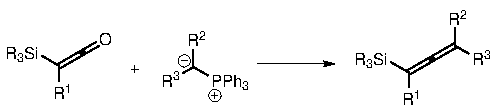
\includegraphics[width=8.2cm,keepaspectratio]{figure1}
%% \sglcolfigure{figure1}
\end{figure}

[\ldots]

\section{Results and Discussion}
Our investigations began with the preparation of substituted silylketenes \CN{1} as substrates for the alkylidenation chemistry. This was carried out under our previously reported conditions for rhodium(II) octanoate-mediated rearrangement of silyl diazoketones \CN{2}, which in turn were prepared by \textit{C}-silylation of the parent diazoketones \CN{3} with triethylsilyl triflate (\cref{scheme:1}). It should be noted that while the alkyl-substituted silylketenes are relatively stable and show little decomposition at room temperature over several days, the (hetero)aromatic-substituted silylketenes are much less robust and should be used quickly or stored in a freezer.

\begin{scheme}
\caption{Synthesis of substituted silylketenes \CN{1}.}
\label{scheme:1}
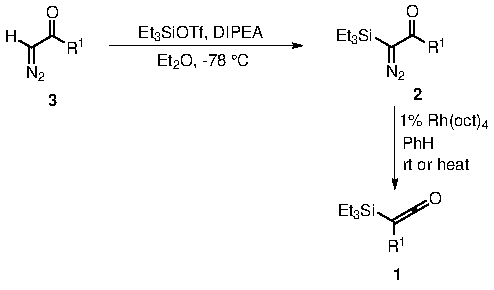
\includegraphics[width=8.2cm,keepaspectratio]{scheme1}
\end{scheme}

[\ldots]

With the requisite silylketenes in hand, attention turned to their reaction with the carboethoxy-stabilised phosphoranes \CN{4} and \CN{5}. At the outset, it was by no means certain that these would react efficiently with substituted silylketenes \CN{1} since it is well documented that nucleophiles attack silylketenes \textit{anti} to the silicon, i.e., the phosphoranes would be approaching from the same side as the \chem{R^1}-substituent. Since in all previous examples this substituent has been a hydrogen atom, the extension to bulkier substituents could not be taken for granted. In the event, however, we were pleased to find that in nearly all cases the desired allenylsilanes were formed in moderate to excellent yield (\cref{scheme:2}, \cref{tab:1}, see \cref{si:1} for full experimental data).
\begin{scheme}
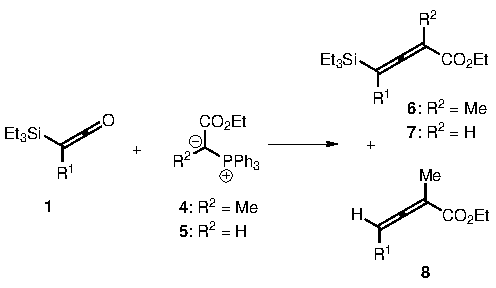
\includegraphics[width=8.2cm,keepaspectratio]{scheme2}
\caption{Reaction of substituted silylketenes with ester-stabilised phosphoranes.}
\label{scheme:2}
\end{scheme}
%%%%%%%%%%%%%%%%%%%%%%%%%%%%%%%%%%%%%%%%%%%%%%%%%%%%%%%%%%%%%%%%%%%%%
%% Tables are a bit special. Only there the \footnote is allowed for
%% Beilstein publications.
%%
%% As for figures and schemes sglcoltabular and dblcoltabular can be
%% used to get tables of the correct width. If you do not want to
%% messure the columns you can use parameter ``X'' of the tabularx
%% package for one column or more to get equal-sized columns.
%%%%%%%%%%%%%%%%%%%%%%%%%%%%%%%%%%%%%%%%%%%%%%%%%%%%%%%%%%%%%%%%%%%%%

\begin{table}
\caption{Reaction of substituted silylketenes with ester-stabilised phosphoranes.}
\label{tab:1}
\begin{dblcoltabularx}{|l|l|l|l|l|X|X|}\hline
\bfseries Entry & \bfseries Ketene & \bfseries Ylide & \bfseries Temp [\celsius] & \bfseries \textit{t} [h] & \bfseries Solvent & \bfseries Yield 6/7 (8)\\\hline
1 & \CN{1a} & \CN{4} & 80 & 24 & PhH & 54\,\%\\\hline
2 & \CN{1a} & \CN{5} & rt & 3  & \CHCL & 60\,\%\\\hline
3 & \CN{1b} & \CN{4} & 110 & 24 & toluene & 45\,\%\\\hline
4 & \CN{1b} & \CN{5} & reflux & 24 & \CHCL & 77\,\%\\\hline
5 & \CN{1c} & \CN{4} & 80 & 24 & PhH & 60\,\%\\\hline
6 & \CN{1c} & \CN{5} & rt & 6  & \CHCL & 81\,\%\\\hline
7 & \CN{1d} & \CN{4} & 110 & 48 & toluene & 22\,\%%
   \footnote{60\,\% of starting material recovered}\\\hline
8 & \CN{1d} & \CN{5} & 80 & 48 & toluene & 78\,\%\\\hline
9 & \CN{1e} & \CN{4} & 80 & 24 & PhH & 55\,\% (7\,\%)\\\hline
10 & \CN{1f} & \CN{4} & 60 & 5 & \CHCL & 44\,\% (3\,\%)\\\hline
11 & \CN{1h} & \CN{4} & rt & 6 & \CHCL & 0\,\% (57\,\%)\\\hline
12 & \CN{1h} & \CN{4} & 50 & 1 & \CHCL & 7\,\% (23\,\%)\\\hline
13 & \CN{1i} & \CN{4} & rt & 10 & \CHCL & 0\,\% (67\,\%)\\\hline
14 & \CN{1i} & \CN{5} & rt & 2 & \CHCL & 98\,\%\\\hline
15 & \CN{1j} & \CN{4} & 80 & 12 & PhH & 74\,\% (19\,\%)\\\hline
\end{dblcoltabularx}
\end{table}

As expected, reactions with the more substituted ylide \CN{4} were significantly slower than those with the parent ylide \CN{5} (compare reaction temperatures and times, entries 1, 3 and 5 versus entries 2, 4 and 6). [...]

%%%%%%%%%%%%%%%%%%%%%%%%%%%%%%%%%%%%%%%%%%%%%%%%%%%%%%%%%%%%%%%%%%%%%
%% The Supporting Information is an essential part of many articles.
%% They are given inside the ``suppinfo'' environment with the
%% \sifile command which gets the following mandatory arguments:
%% #1: File name
%% #2: File type
%% #3: Descriptive File title
%% A long description can be given using the optional argument.
%%
%% You can label each entry and reference it in the text.
%%%%%%%%%%%%%%%%%%%%%%%%%%%%%%%%%%%%%%%%%%%%%%%%%%%%%%%%%%%%%%%%%%%%%
\begin{suppinfo}
Supporting information features copies of \HNMR spectra of silylated diazoketones \CN{2} and silylketenes \CN{1}, plus \chem{{}^1H} and \CNMR spectra of allenylsilanes \CN{6}, \CN{7}, and \CN{14}--\CN{19}.
\sifile{S1.pdf}{PDF}{Experimental part}\label{si:1}
\sifile{S2.pdf}{PDF}{NMR spectra of compounds \CN{1}, \CN{2}, \CN{6} and \CN{7}}
\sifile{S3.pdf}{PDF}{NMR spectra of compounds \CN{14--19}}
\end{suppinfo}

%%%%%%%%%%%%%%%%%%%%%%%%%%%%%%%%%%%%%%%%%%%%%%%%%%%%%%%%%%%%%%%%%%%%%
%% The sections "Acknowledgements" and "Funding" can be given in all
%% manuscripts.
%% This should be done within the environments ``acknowledgements''
%% and ``funding'', which will produce the correct section titles.
%%%%%%%%%%%%%%%%%%%%%%%%%%%%%%%%%%%%%%%%%%%%%%%%%%%%%%%%%%%%%%%%%%%%%
\begin{acknowledgements}
We acknowledge Prof. H. Vlassov for the helpful discussions of the results and J. Martin for assistance with the synthesis.
\end{acknowledgements}

\begin{funding}
The following sources of funding are acknowledged: National Natural Science Foundation of China (S.P.M.; Grant Nos. 51502240, 11674273, U1856203), Wellcome Trust (S.P.M., Award No. 094542/Z/12/Z, EPSRC (P.C.D.; Grant No. GR/L60135/01 (PCD)), and both authors thank the generous research funding from Pfizer for financial support.
\end{funding}

%%%%%%%%%%%%%%%%%%%%%%%%%%%%%%%%%%%%%%%%%%%%%%%%%%%%%%%%%%%%%%%%%%%%%
%% The appropriate \bibliography command should be placed here.
%% Notice that the class file automatically sets \bibliographystyle
%% and also names the section correctly.
%%%%%%%%%%%%%%%%%%%%%%%%%%%%%%%%%%%%%%%%%%%%%%%%%%%%%%%%%%%%%%%%%%%%%
\bibliography{beilstein-template}

%%%%%%%%%%%%%%%%%%%%%%%%%%%%%%%%%%%%%%%%%%%%%%%%%%%%%%%%%%%%%%%%%%%%%
%% That's it. Ending the document finishes the article. Happy TeXing!
%%%%%%%%%%%%%%%%%%%%%%%%%%%%%%%%%%%%%%%%%%%%%%%%%%%%%%%%%%%%%%%%%%%%%
\end{document}
